
\section{Method}
In this section, we introduce our proposed YOLOv13 method. In Sec.~\ref{sec:overall}, we introduce the overall network architecture of our proposed model. Then, the detailed ideology and structure of our proposed hypergraph-based adaptive correlation enhancement mechanism and the full-pipeline aggregation-and-distribution paradigm are presented in Sec.~\ref{sec:HyperACE} and Sec.~\ref{sec:fullpad}, respectively. Finally, in Sec.~\ref{sec:dsc3k}, we introduce the architecture of our proposed lightweight feature extraction blocks.

\subsection{Overall Architecture}
\label{sec:overall}
Previous YOLO series follow the ``Backbone $\to$ Neck $\to$ Head" computational paradigm, which inherently constrains the adequate delivery of information flow. In contrast, our model enhances the traditional YOLO architecture by achieving a \textbf{Full}-\textbf{P}ipeline feature \textbf{A}ggregation-and-\textbf{D}istribution (\textbf{FullPAD}) through the \textbf{Hyper}graph-based \textbf{A}daptive \textbf{C}orrelation \textbf{E}nhancement (\textbf{HyperACE}) mechanism. Thus, our proposed method achieves fine‑grained information flow and representation synergy throughout the network, which can improve gradient propagation and significantly enhance detection performance. Specifically, as shown in Fig.~\ref{fig:framework}, our YOLOv13 model first extracts multi-scale feature maps $B_1, B_2, B_3, B_4, B_5$ using a backbone network similar to previous works, but in which the large-kernel convolutions are replaced with our proposed lightweight DS-C3k2 blocks. Then, different from traditional YOLO methods that directly input $B_3$, $B_4$, and $B_5$ into the neck network, our method gathers and forwards these features into the proposed HyperACE module, achieving cross-scale cross-position features high-order correlation adaptive modeling and feature enhancement. Subsequently, our FullPAD paradigm leverages three separate tunnels to distribute the correlation-enhanced feature to the connection between the backbone and neck, the internal layers of the neck, and the connection between the neck and head, respectively, for better information flow. Finally, the output feature maps of the neck are forwarded into detection heads to achieve multi‑scale object detection. 

\subsection{Hypergraph-Based Adaptive Correlation Enhancement}
\label{sec:HyperACE}

To achieve efficient and robust cross‐scale cross‐position correlation modeling and feature enhancement, we propose a hypergraph-based adaptive correlation enhancement mechanism. As shown in Fig.~\ref{fig:framework}, HyperACE contains two core components, \ie, the global high‐order perception branch based on the C3AH module, in which high‐order visual correlations are modeled with linear complexity using adaptive hypergraph computation, and the local low‐order perception branch based on the DS‐C3k block. In the following subsections, we will introduce the adaptive hypergraph computation, the C3AH module, and the overall design of the HyperACE, respectively.

\subsubsection{Adaptive Hypergraph Computation}
To effectively and efficiently model the high-order correlation in visual features and achieve correlation-guided feature aggregation and enhancement, we propose a novel adaptive hypergraph computation paradigm. Different from traditional hypergraph modeling methods that use manual pre-defined parameters to construct hyperedges based on feature similarity, our proposed method adaptively learns the participation degree of each vertex for each hyperedge, making this computational paradigm more robust and efficient. The traditional hypergraph computing paradigm is more applicable to non-Euclidean data, \eg, social networks, since it contains explicit connection relationships, while our adaptive hypergraph computing paradigm is more conducive to computer vision tasks. 

Specifically, our proposed adaptive hypergraph is defined as $\mathcal{G}= \{\mathcal{V}, \mathcal{A}\}$, where $\mathcal{V}$ is the vertex set, and $\mathcal{A}$ is the adaptive hyperedge set. In an adaptive hypergraph, each hyperedge connects all vertices, where each vertex participates in the hyperedge with a continuous and differentiable contribution degree. Therefore, different from the traditional hypergraph which uses an incidence matrix $H \in \{0,1\}^{N \times M}$ for representation, our adaptive hypergraph is represented using a continuous participation matrix $A \in [0,1]^{N \times M}$, where $N$ and $M$ are the number of vertices and hyperedges, respectively. $A_{i,m}$ denotes the participation degree of vertex $i$ in hyperedge $m$. Accordingly, our adaptive hypergraph computation paradigm consists of two stages, \ie, adaptive hyperedge generation and hypergraph convolution, as shown in Fig.~ \ref{fig:hyperace}.
\input{sections/figs/fig4-HyperACE}

\textbf{Adaptive Hyperedge Generation}.
The adaptive hyperedge generation stage focuses on dynamically modeling correlations from input visual features to generate hyperedges and estimate the participation degree of each vertex to each hyperedge. Specifically, let $X=\bigl\{x_i \in \mathbb{R}^C \mid i = 1, \dots, N\bigr\}$ denote the vertex features, where $C$ is the number of feature channels. Our proposed method first uses global average pooling and max pooling to generate context vectors $f_{\mathrm{avg}}$ and $f_{\mathrm{max}}$, respectively. Then, the context vectors are concatenated to obtain global vertex context $f_{\mathrm{ctx}}$, \ie, 
\begin{equation}
    f_{\mathrm{ctx}}
= \begin{pmatrix} f_{\mathrm{avg}} \\[4pt] f_{\mathrm{max}} \end{pmatrix}
\in \mathbb{R}^{2C}.
\end{equation}
Subsequently, a mapping layer $\phi: \mathbb{R}^{2C} \to \mathbb{R}^{M \times C}$ is leveraged to generate the global offset $\Delta P$ from the vertex context, \ie, $\Delta P = \phi(f_{\mathrm{ctx}})$, where $M$ is the number of hyperedges. The global offset is then added with a learnable global prototype \(P_0 \in \mathbb{R}^{M \times C}\) to obtain $M$ dynamic hyperedge prototypes $P$, \ie, $P = P_0 + \Delta P$. These prototypes represent potential visual correlations within the scene. To calculate the participation degree of each vertex, another projection layer is leveraged to generate the vertex query vector $z_i$ from vertex feature $x_i$, \ie,
\begin{equation}
    z_i = W_{\mathrm{pre}}\,x_i \in \mathbb{R}^C,
\end{equation}
where \(W_{\mathrm{pre}}\) is the weight matrix. 

To further increase feature diversity, we introduce a multi‐head mechanism to split \(z_i\) into \(h\) subspaces $\{ \hat z_i^\tau \in \mathbb{R}^{d_h}\}_{\tau=1}^h$ along the feature dimension, where $d_h = C/h$, and we similarly split each hyperedge prototype into \(h\) subspaces $\{\hat p_m^\tau \in \mathbb{R}^{d_h}\}_{\tau=1}^h$. Then, in the \(\tau\)‐th subspace, the similarity between the $i$-th vertex query vector and the $m$-th prototype is computed:
\begin{equation}
    s_{i,m}^\tau = \frac{\langle \hat z_i^\tau, \hat p_m^\tau\rangle}{\sqrt{d_h}}.
\end{equation}
Thus, the overall similarity is defined as the average of all subspace similarities, \ie, $\bar s_{i,m} = \frac{1}{h} \sum_{\tau=1}^h s_{i,m}^\tau$.
Finally, we use the similarity between the vertex query vector and the prototype as the contribution of the vertex to the hyperedge, and normalize across vertices to obtain the continuous participation matrix \(A\), formulated as:
\begin{equation}
    A_{i,m}
= \frac{\exp\bigl(\bar s_{i,m}\bigr)}
       {\displaystyle\sum_{j=1}^{N}\exp\bigl(\bar s_{j,m}\bigr)}.
\end{equation}

\textbf{Hypergraph Convolution}.
After the adaptive hyperedges are generated, the hypergraph convolution is conducted to achieve feature aggregation and enhancement. Specifically, in the hypergraph convolution, each hyperedge first collects features from all vertices and applies a linear projection to form the hyperedge feature. Then, the hyperedge features are disseminated back to the vertices to update their representations. Formally, this process can be defined as:
\begin{equation}
    \begin{aligned}
        f_{m} &= \sigma\Bigl(W_{e}\sum_{i=1}^{N} A_{i,m}\,x_{i}\Bigr)\\
        \widetilde x_{i} &= \sigma\Bigl(W_{v}\sum_{m=1}^{M} A_{i,m}\,f_{m}\Bigr)
    \end{aligned},
\end{equation}
where $i=1,\dots,N$ is the vertex index, $m=1,\dots,M$ is the hyperedge index, $W_{e}$ and $W_{v}$ denote the hyperedge and vertex projection weights, respectively, and $\sigma$ is the activation function.

\subsubsection{C3AH for Adaptive High-Order Correlation Modeling}
Based on our proposed adaptive hypergraph computation paradigm, we further propose the C3AH block to efficiently capture high-order semantic interactions. Specifically, as shown in Fig.~\ref{fig:framework}, the C3AH block retains the CSP bottleneck branch-split mechanism while integrating an adaptive hypergraph computation module, enabling global high-order semantic aggregation across spatial positions.

Let the input feature map of C3AH block be $X_{\mathrm{in}}\in\mathbb{R}^{C_{\mathrm{in}}\times H\times W}$. We first apply two $1\times1$ convolutional layers to project it into the same hidden dimension,\ie,
\begin{equation}
    X = \text{Conv}_{1\times1}(X_{\text{in}}),\quad
X_{\text{lateral}} = \text{Conv}_{1\times1}(X_{\text{in}}),
\end{equation}
where $X,\,X_{\mathrm{lateral}}\in\mathbb{R}^{C\times H\times W}$ and $C=\lfloor e\,C_{\mathrm{in}}\rfloor$, $e$ is the bottleneck compression ratio. $X$ and $X_{\text{lateral}}$ are used for adaptive hypergraph computation and lateral connection, respectively.

Then, $X$ is flattened as the vertex features and is sent to the adaptive hypergraph computation module, denoted as AHC, to obtain correlation-enhanced features:
\begin{equation}
    X_{h} = \mathrm{AHC}(X).
\end{equation}
Finally, $X_{h}$ and $X_{\mathrm{lateral}}$ are concatenated along the channel dimension and then fused by a $1\times1$ convolutional layer to obtain the output of C3AH block.

\subsubsection{Structure of HyperACE}
HyperACE takes multi‐scale features as input to achieve efficient visual correlation modeling and feature enhancement. Specifically, HyperACE first takes the feature maps $B_3$, $B_4$, and $B_5$ from the last three stages of the backbone as input, then resizes $B_3$ and $B_5$ to the same spatial size as \(B_4\), and aggregates them via a \(1\times1\) convolutional layer to obtain the fused feature $X_b$. Subsequently, \(X_b\) is split along the channel dimension into three feature groups, denoted as $X_b^h \in \mathbb{R}^{C_h\times H\times W}$, $X_b^l \in \mathbb{R}^{C_l\times H\times W}$, and $X_b^s \in \mathbb{R}^{C_s\times H\times W}$, respectively. $X_b^h$, $X_b^l$, and $X_b^s$ are used for global high‑order correlation modeling, local low‑order correlation modeling, and shortcut connection, respectively.

In the high‑order correlation modeling branch, $X_b^h$ is forwarded into $K$ parallel C3AH blocks to explore various latent high-order correlations and obtain enhanced features, \ie, 
\begin{equation}
    \bigl\{X_h^{(k)} = \text{C3AH}_k(X_b^h)\mid k=1,\dots,K\bigr\}.
\end{equation}
These \(K\) enhanced features are then concatenated along the channel dimension to obtain the output of the high‑order correlation modeling branch $X_h$, \ie,
\begin{equation}
    X_h = \mathrm{Concat}\bigl(X_h^{(1)},\,X_h^{(2)},\,\dots,\,X_h^{(K)}\bigr).
\end{equation}
In the local low‑order correlation modeling branch, we use $L$ stacked DS‑C3k modules to capture fine‑grained local information, \ie, 
\begin{equation}
    X_l
= \text{DS-C3k}\bigl(X_b^l\bigr).
\end{equation}
The shortcut branch directly retains the original visual information, \ie, $X_s = X_b^s$.

Finally, the outputs of three branches are concatenated along the channel dimension and fused by a \(1\times1\) convolutional layer to obtain the final output of HyperACE, formulated as:
\begin{equation}
    Y = \mathrm{Conv}_{1\times1}\!\bigl(\mathrm{Concat}(X_h,\,X_l,\,X_s)\bigr).
\end{equation}

Our proposed HyperACE fully leverages the parallel global high‑order correlation modeling branch and the local low‑order correlation modeling branch, while preserving shortcut information, achieving complementary multi‑level visual correlation perception across global-local and high-low orders.

\subsection{Full-Pipeline Aggregation-and-Distribution Paradigm}
\label{sec:fullpad}
To fully utilize the correlation-enhanced features obtained from HyperACE, we further introduce the FullPAD paradigm. Specifically, FullPAD collects multi‐scale feature maps from the backbone and forwards them into HyperACE, and then redistributes the enhanced features to various locations throughout the pipeline via different FullPAD tunnels, as is shown in Fig.~\ref{fig:framework}. This design enables fine‐grained information flow and representation synergy, significantly improving gradient propagation and enhancing detection performance.

In practice, after the correlation-enhanced feature $Y$ is obtained from $B_3$, $B_4$, $B_5$ using HyperACE, FullPAD resizes $Y$ to the spatial resolution of each stage and adjusts its channel dimension using a \(1\times1\) convolutional layer, \ie, 
\begin{equation}
    H_i = \text{Conv}_{1\times1}\bigl(\text{Resize}(Y \leftarrow \mathrm{size}(B_i))\bigr),
\quad i \in \{3,4,5\}.
\end{equation}
Then, for an arbitrary feature map \(F_i\) at stage \(i\), a gated fusion is leveraged to achieve information flow and fusion:
\begin{equation}
    \widetilde{F_i}= F_i+\gamma H_i,
\end{equation}
where \(\gamma\) is a learnable scalar parameter that adaptively balances the contribution of the correlation‐enhanced feature and original feature. In practice, FullPAD transmits the output correlation-enhanced features to seven different destinations via three different tunnels, as shown in Fig.~\ref{fig:framework}.

Based on our proposed FullPAD paradigm, correlation-enhanced features are effectively integrated into different stages of the entire pipeline, enabling the model to fully utilize the visual correlation information to perceive complex scenarios effectively.


\subsection{Model Lightweighting with Depth-Separable Convolution}
\label{sec:dsc3k}

In our proposed YOLOv13, we leverage large‐kernel depthwise-separable convolution (DSConv) as the basic unit to design a series of lightweight feature extraction blocks, as shown in Fig.~\ref{fig:dsblock}, which significantly reduces the number of parameters and computational complexity without compromising model performance.

\textbf{DSConv.} The DSConv block first applies a standard depthwise separable convolutional layer to extract features, and then leverages batch normalization and SiLU activation to obtain the output, \ie,
\begin{equation}
    X_{\mathrm{DS}}
=\mathrm{SiLU}\bigl(\mathrm{BN}\bigl(\mathrm{DSConv}(X_{\mathrm{in}})\bigr)\bigr).
\end{equation}

\textbf{DS‐Bottleneck.} In the DS‐Bottleneck block, we cascade two DSConv blocks, among which the first block is a fixed $3\times3$ depthwise‐separable convolution, and the second block is a large‐kernel ($k\times k$) depthwise‐separable convolution, \ie,
\begin{equation}
    X_{\mathrm{DS2}}
= \mathrm{DSConv}_{k\times k}\bigl(\mathrm{DSConv}_{3\times3}(X_{\mathrm{in}})\bigr).
\end{equation}
Meanwhile, if the input and output have the same number of channels, a residual skip connection will be added to preserve low‐frequency information.
\begin{figure}[!tbp]
    \centering
    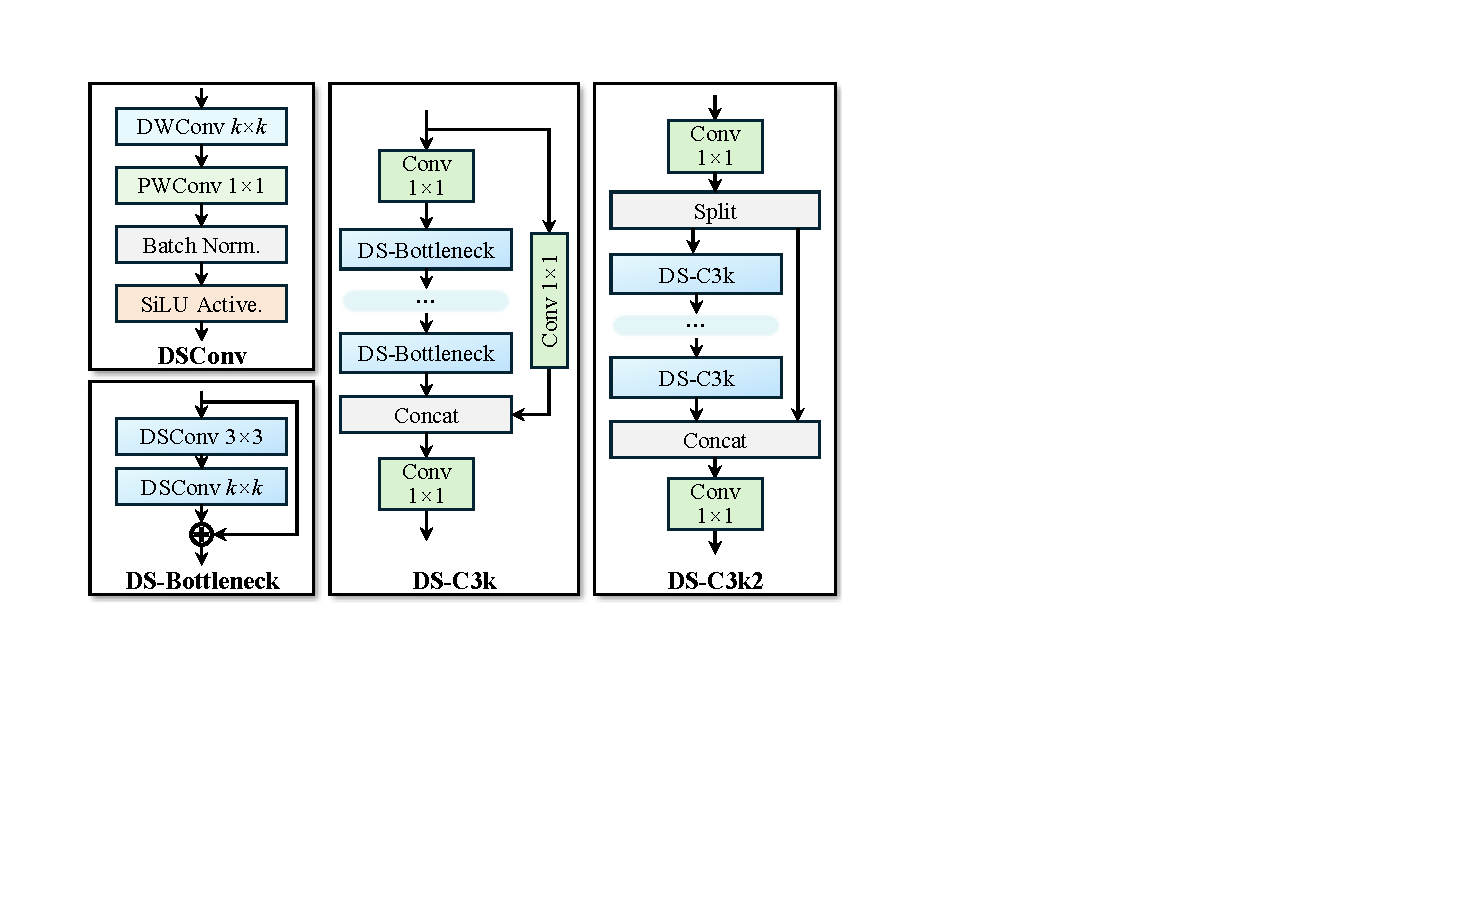
\includegraphics[width=1\linewidth]{figures/dsblocks.pdf}
    \vspace{-0.5cm}
    \caption{Detailed architecture of our proposed DS-series blocks.}
    \vspace{-0.4cm}
    \label{fig:dsblock}
\end{figure}

\textbf{DS-C3k.} The DS‐C3k block inherits from the standard CSP-C3 structure~\cite{yolov5}. Specifically, the input feature is first forwarded into a $1\times1$ convolutional layer to reduce feature channels, and is then processed by $n$ cascaded DS‐Bottleneck blocks. Meanwhile, a lateral $1\times1$ convolutional branch is applied to the input feature. Finally, the features from two branches are concatenated along the channel dimension, and a $1\times1$ convolutional layer is leveraged to restore the feature channels. This design retains the cross‐channel branching of CSP structure while integrating depthwise‐separable lightweight bottlenecks.

\textbf{DS-C3k2.} The DS‐C3k2 block is derived from the C3k2 structure~\cite{yolo11}. Specifically, a $1\times1$ convolutional layer is first applied to unify the channels. Then, the features are split into two parts, with one part fed into multiple DS-C3k modules and the other passed through a shortcut connection. Finally, the outputs are concatenated and fused with a $1\times1$ convolutional layer.




As shown in Fig~\ref{fig:framework}, our proposed YOLOv13 model extensively uses DS-C3k2 blocks as the basic feature extraction module in both the Backbone and the Neck. In HyperACE, we leverage the DS‐C3k block as the low‐order feature extractor. This design achieves up to 30\% parameter reduction and up to 28\% GFLOPs reduction across all YOLOv13 model sizes.

Using our proposed YOLOv13 model, the latent correlations in visual features are adaptively modeled, and by fully propagating the correlation-enhanced features throughout the full pipeline, accurate and efficient object detection in complex scenes can be achieved.

% By using our proposed YOLOv13 model to adaptively model latent correlations in scene visual features and to fully propagate the enhanced features throughout the pipeline, we enable accurate and efficient object detection in complex scenes.